\documentclass[main.tex]{subfiles}
\renewcommand{\epsilon}{\varepsilon}
\begin{document}
\section{Quelques chiffres}
\emph{Cf poly}

\emph{Beaucoup de donnée disponible dans le poly, encore plus sur le site de RTE}.
\begin{defin}
  Le \emph{facteur de charge} ou facteur d'utilisation d'une centrale électrique est le rapport entre l'énergie électrique effectivement produite sur une période donnée et l'énergie qu'elle aurait produite si elle avait fonctionné à sa puissance nominale durant la même période.
\end{defin}

\section{Caractérisation du vent}
De façon à étudier le potentiel éolien d'un site il convient de connaitre la source d'énergie: le vent. Ces renseignements sont donnés par:
\begin{itemize}
\item la rose des vents
\item la distribution des vitesses
\item La dépendance en fonction de l'altitude
\end{itemize}
\subsection{La rose des vents}
\subsection{La distribution des vitesses}
\subsection{Dépendances de la vitesse du vent avec l'altitude}
Les frottement avec la surface terrestre font que la vitesse du varie en fonction de l'altitude. La loi empirique suivante permet de prendre en compte cette dépendance.
\[
  \frac{V}{V_{ref}}= \left(\frac{H}{H_{ref}}\right)^\alpha
\]
Avec
\begin{description}
\item[H] hauteur
\item[$\alpha$] coefficient permettant de prendre en compte la rugosité du terrain.
  \begin{center}
    \begin{tabular}[H]{|c|c|}
      \hline
      Mer calme  & $\alpha = 0,09$ \\
      \hline
      prairie & $\alpha = 0,16$\\
      \hline
  \end{tabular}
\end{center}
\end{description}
\subsection{Énergie cinétique d'une colonne de vent}
L'énergie cinétique d'une colonne de vent de masse $m$ se déplaçant à la vitesse $V$ s'écrit:
\[
E_c = \frac{1}{2}m.V^2
\]
\begin{figure}[H]
  \centering
  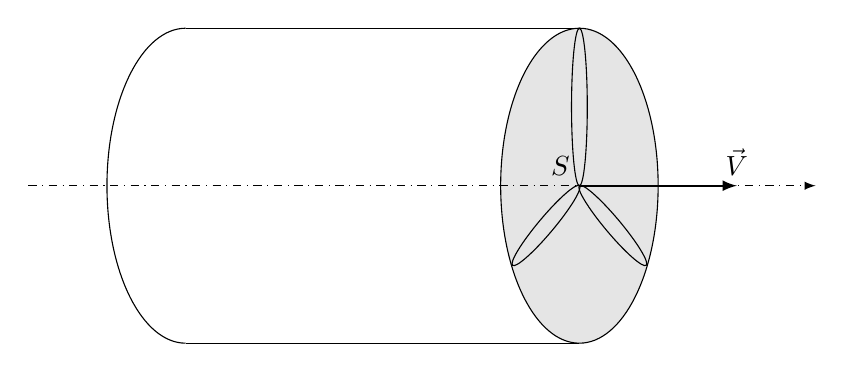
\begin{tikzpicture}
    \draw[fill=gray!20] (0,0) ellipse (1 and 2) node[above left]{$S$};
    \draw (0,2) -- ++(-5,0) (0,-2) -- ++(-5,0);
    \draw (-5,-2) arc(-90:90:-1 and 2);
    \draw[dash dot,-latex] (-7,0) -- (3,0);
    \draw[thick,-latex](0,0) -- ++(2,0) node[above]{$\vec{V}$};
    \draw (0,1) ellipse (0.1 and 1);
    \draw[rotate={140}] (0,0.66) ellipse (0.1 and 0.66);
    \draw[rotate={220}] (0,0.66) ellipse (0.1 and 0.66);

  \end{tikzpicture}
  \caption{Colonne de vent}
\end{figure}
En supposant qu'en sortie de l'éolienne la vitesse de cette colonne soit nulle , il serait possible de récupérer dans l'intervalle de temps $dt$ l'énergie élémentaire:
\[
  \d E_c= \frac{1}{2}\d mV^2
\]
où $\d m$ représente la masse ayant traversé la surface $S$ pendant le temps $\d t$.Soit $\d m = \rho SV\d t$ avec $\rho$\SI{1,225}{\kg\per\m^3} masse volumique de l'air dans les conditions normale de pression et de température.
\[
  \d E_c= \frac{1}{2}\rho SV^3 \d t
\]
On fournit alors une puissance:
\[
  P_{E_c} = \frac{1}{2}\rho SV^3
\]
\subsection{Potentiel éolien d'un site}
Connaissant l'histogramme des vitesses sur un site il est possible de calculer la contribution pour que chaque vitesse de vent à l'énergie cinétique sur 1 an. Le principe de calcul est le suivant:
\begin{itemize}
\item Un vent de \SI{5}{\m\per\s} souffle 22\% du temps,soit \SI{1927}{h/an}.
\item La puissance par unité de surface s'écrit : $\frac{P_{E_c}}{S} = \frac{1}{2}\rho V^3 = $\SI{76,5}{W\per\m^2}
\item La contribution de cette vitesse à l'énergie est donc:
\[
  \left(\frac{W_{E_c}}{S}\right)_{V=5m/s)} = \text{\SI{150}{kWh/m^2/an}}
\]
Pour avoir l'énergie théorique sur un an et par unité de surface, il suffit de sommer les différentes vitesses

\[
  \frac{W_{E_c}}{S} = \text{\SI{821}{kWh/m^2/an}}
\]
pour une éolienne balayant une surface de 100 $m^2$, l'énergie de la veine de vent sur un an serait $W_{E_c} =$ \SI{82100}{kWh}.
Comme le montrerons les parties suivantes, l'énergie convertie sera beaucoup faible et représentera environ 50\% de l'énergie du vent.
\end{itemize}
\subsection{Potentiel éolien en France}
\emph{bullshit.}

\section{Les différents types de turbines}
\emph{bullshit}
\section{Conversion d'énergie cinétique, mécanique}
\subsection{Limite de Betz}
Dans le chapitre concernant le vent, nous avons montré en supposant qu'en sortie de l'hélice la vitesse de la colonne de vent soit nulle , qu'il serait possible de fournir une puissance:$ P_{E_c} =\frac{1}{2}:\rho SV^3$.
Les particules constituant l'air ne pouvant disparaître en sortie de l'hélice il y  aura une limite à cette puissance. Albert Betz (1919) a démontré en supposant l'écoulement de l'air incompressible que le transfert est limité.
\begin{prop}[Limite de Betz]
  En considérant un écoulement incompressible sur la turbine on peux \emph{au maximum} extraire de la puissance du vent:
\[
P_{max} = \frac{16}{27}P_{E_c}
\]
\end{prop}
\begin{figure}[H]
  \centering
  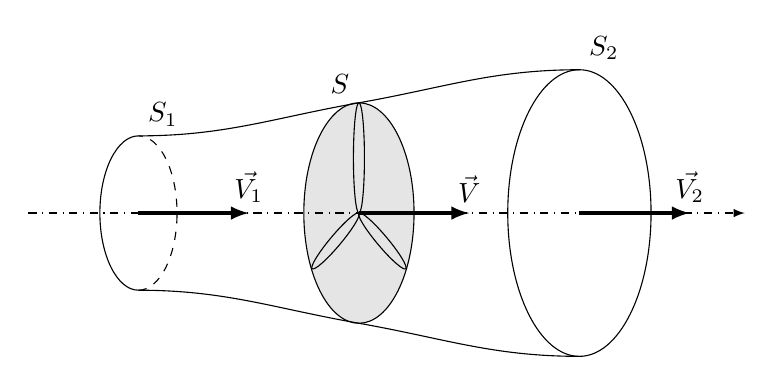
\begin{tikzpicture}[scale=0.7]
    \draw[fill=gray!20] (0,0) ellipse (1 and 2) (0,2)node[above left]{$S$};
    \draw (-4,-1.4) arc(-90:90:-0.7 and 1.4) node[above right]{$S_1$};
    \draw[dashed] (-4,-1.4) arc(-90:90:0.7 and 1.4);
    \draw (-4,1.4) to[out=0,in=190] (0,2)to[out=10,in=180] (4,2.6);
    \draw (-4,-1.4) to[out=0,in=170] (0,-2)to[out=-10,in=180](4,-2.6);
    \draw (4,0) ellipse (1.3 and 2.6)(4,2.6) node[above right]{$S_2$};
    \draw[dash dot,-latex] (-6,0) -- (7,0);
    \draw[very thick,-latex](0,0) -- ++(2,0) node[above]{$\vec{V}$};
    \draw[very thick,-latex](-4,0) -- ++(2,0) node[above]{$\vec{V_1}$};
    \draw[very thick,-latex](4,0) -- ++(2,0) node[above]{$\vec{V_2}$};
    \draw (0,1) ellipse (0.1 and 1);
    \draw[rotate={140}] (0,0.66) ellipse (0.1 and 0.66);
    \draw[rotate={220}] (0,0.66) ellipse (0.1 and 0.66);
  \end{tikzpicture}
  \caption{Veine de vent à la traversée de l'aéromoteur}
\end{figure}

  \begin{minipage}[t]{0.5\textwidth}
      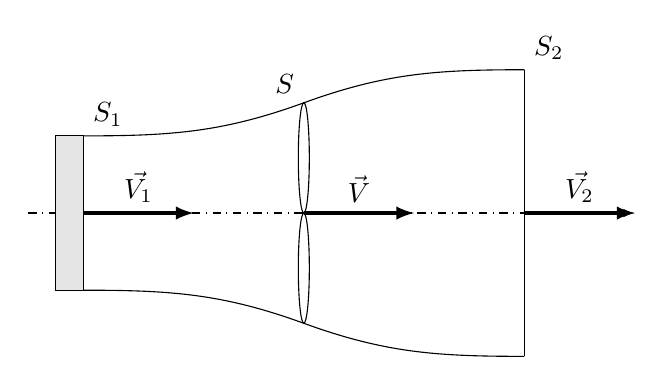
\begin{tikzpicture}[scale=0.7]
    \draw (0,2)node[above left]{$S$};
    \draw (0,1) ellipse(0.1 and 1) (0,-1) ellipse(0.1 and 1);
    \draw (-4,1.4) node[above right]{$S_1$} -- (-4,-1.4);
    \draw (-4.5,1.4) -- (-4,1.4) to[out=0,in=200] (0,2)to[out=20,in=180] (4,2.6);
    \draw (-4.5,-1.4) -- (-4,-1.4) to[out=0,in=160] (0,-2)to[out=-20,in=180](4,-2.6);
    \draw (4,2.6) node[above right]{$S_2$} -- (4,-2.6);
    \draw[dash dot,-latex] (-5,0) -- (6,0);
    \draw[very thick,-latex](0,0) -- ++(2,0) node[midway,above]{$\vec{V}$};
    \draw[very thick,-latex](-4,0) -- ++(2,0) node[midway,above]{$\vec{V_1}$};
    \draw[very thick,-latex](4,0) -- ++(2,0) node[midway,above]{$\vec{V_2}$};
    \draw[fill=gray!20] (-4.5,-1.4) rectangle (-4,1.4);

  \end{tikzpicture}\\
  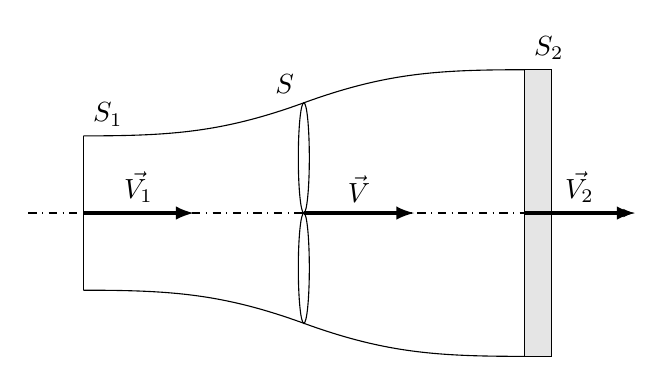
\begin{tikzpicture}[scale=0.7]
      \draw (0,2)node[above left]{$S$};
      \draw (0,1) ellipse(0.1 and 1) (0,-1) ellipse(0.1 and 1);
    \draw (-4,1.4) node[above right]{$S_1$} -- (-4,-1.4) (4.5,2.6) -- (4.5,-2.6);
    \draw (-4,1.4) to[out=0,in=200] (0,2)to[out=20,in=180] (4,2.6) -- (4.5,2.6);
    \draw (-4,-1.4) to[out=0,in=160] (0,-2)to[out=-20,in=180](4,-2.6)  -- (4.5,-2.6);
    \draw (4,2.6) node[above right]{$S_2$} -- (4,-2.6);
\draw[fill=gray!20] (4.5,2.6) rectangle (4,-2.6);
    \draw[dash dot,-latex] (-5,0) -- (6,0);
    \draw[very thick,-latex](0,0) -- ++(2,0) node[midway,above]{$\vec{V}$};
    \draw[very thick,-latex](-4,0) -- ++(2,0) node[midway,above]{$\vec{V_1}$};
    \draw[very thick,-latex](4,0) -- ++(2,0) node[midway,above]{$\vec{V_2}$};
  \end{tikzpicture}
\end{minipage}%
  \begin{minipage}{0.45\linewidth}
    \begin{itemize}
    \item À l'instant $t$ la quantité de mouvement de la veine de vent s'écrit:
      \begin{align*}
      p(t) &= p_{ABEF} + p_{BCDE} \\
           &= d_n v_1(t) + p_{BCDE}
      \end{align*}
    \item À l'instant $t+\d t$ la quantité de mouvement de la veine de vent s'écrit:
      \begin{align*}
      p(t) &= p_{CGDH} + p_{BCDE} \\
           &= d_n v_2(t) + p_{BCDE}
      \end{align*}
    \end{itemize}
  \end{minipage}
  
  \vspace{1em}
  Le débit se conservant et l'écoulement étant supposé incompressible, la masse élementaire $\d m$ est la masse qui traverse la surface $S$ pendant $\d t$.Soit:
  \[
    \deriv[m]{t} = \rho S v = \rho S_1v_1 = \rho S_2 v_2
  \]
  En régime permanent, la variation de la quantité de mouvement durant le temps $\d t$ s'écrit:
  \[
    \d p = p(t+\d t) -p(t) = \rho S v \d t (v_2-v_1)
  \]
  On en déduit que la puissance cédée à l'hélice est donnée par la relation:
  \[
    P = \rho S v^2 (v_2-v_1)
  \]
  Cette puissance peut aussi être déterminer en effectuant un bilan d'énergie sur la veine de vent. La variation d'énergie cinétique entre les instants $t$ et $t+\d t$ s'écrit:
  \[
    \d E_{c} = \frac{1}{2}\d m (v_2^2-v_1^2)
  \]
  Soit
  \[
    P = \frac{\rho S v}{2}(v_2^2-v_1^2)
  \]
  En égalisant les deux expressions de la puissance transférée à l'hélice
  \[
    \rho S v^2 (v_2-v_1) = \frac{\rho S v}{2}(v_2^2-v_1^2) \implies \boxed{v =\frac{v_1+v_2}{2}}
  \]
  On en déduit une autre expressions de la puissance ne faisant intervenir que les vitesses avant et après l'hélice.
  \[
    P= \frac{\rho S}{4} (v_1+v_2) (v_2^2-v_1^2)
  \]
  pour une vitesse $v_1$ donnée cette puissance passe par un maximum quand $\deriv[P]{v_2} = 0$. Et le maximum est donnée par l'expression:

\[
  P = -\frac{16}{27}\underbracket{\frac{\rho S v_1^3}{2} }_{P_{incident}} \text{ pour } v_2 = \frac{1}{3}v_1
\]

\subsection{Théorie Simplifiée de la pale}
On considère une hélice constituée de pales formée de plaques. On note:
\begin{itemize}
\item $v$ la vitesse du vent réel.
\item $\Omega$ la vitesse de rotation de l'hélice.
\end{itemize}

On cherche à détermioner la contribution à la puissance et au couple moteur de l'élement de pale situé à une distance $r$ de l'axe de rotation.

% schéma dégueu.

Pour ce tronçon élementaire, on note :
\begin{itemize}
\item $l$ : largeur
\item $\d r$ : longueur
\item $\beta$ : angle de calage
\end{itemize}

% schéma pale
\begin{figure}[H]
  \centering
  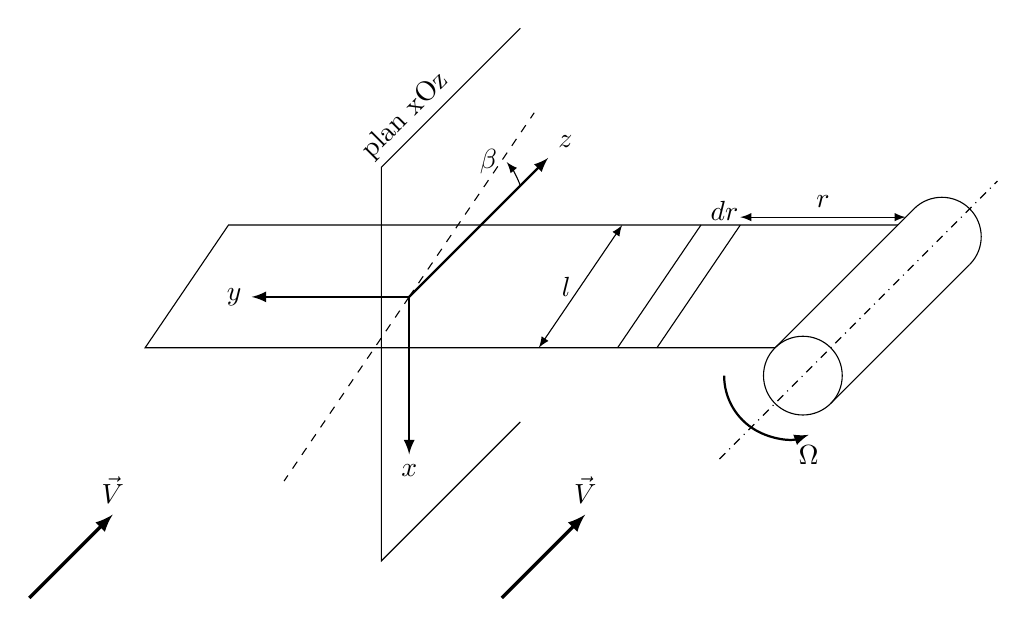
\begin{tikzpicture}
    [z= {(-0.353cm,-0.353cm)}, y={(0cm,1cm)}, x={(1cm,0cm)}]
    \def\dep{(0,0,-5)}
    \draw[dash dot] (0,0,3) -- (0,0,-7);
    \draw (0,0) circle (0.5);
    \draw (135:0.5) -- ++\dep arc(135:-45:0.5);
    \draw (-45:0.5) -- ++\dep;
    \draw (135:0.5) -- ++(-8,0,0)-- ++(0,0.5,-3) -- ++(8.5,0,0);
    \draw[-latex,thick] (-5,1,0) coordinate(O) -> ++(0,0,-5) node[above right]{$z$};
    \draw[-latex,thick] (O) -> ++(0,-2,0)node[below]{$x$};
    \draw[-latex,thick] (O) -> ++(-2,0,0) node[left]{$y$};
    \draw (-5,3,1) coordinate(O2)--  ++(0,0,-5) node[midway ,above=1em,rotate=45,anchor=east]{plan xOz};
    \draw (O2) -- ++(0,-5,0) -- ++(0,0,-5);
    \draw[dashed] (O) -- ++(0,0.75,-4.5) (O)-- ++(0,-0.75,4.5);
    \draw[-latex] (O) ++(0,0,-4) arc(20:40:1) node[above,left]{$\beta$} ;
    \draw[latex-latex] (135:0.5) ++(-3,0,0) -- ++(0,0.5,-3) node[midway, left]{$l$};
    \draw (135:0.5) ++(-2,0,0)coordinate(A) -- ++(0,0.5,-3)node[above=0.5em ,right]{$dr$}
    (A) ++(0.5,0,0) -- ++(0,0.5,-3) coordinate(B);
    \draw[latex-latex] (B)++(0,0.1,0) -- ++(2.1,0,0) node[midway,above]{$r$};

    \draw[latex-,very thick] (-7,0,5)node[above ]{$\vec{V}$} -- ++(0,0,3);
    \draw[latex-,very thick] (-1,0,5)node[above ]{$\vec{V}$} -- ++(0,0,3);

    \draw[-latex,thick] (-1,0,0) arc(180:290:0.8) node[below]{$\Omega$};
  \end{tikzpicture}

  \caption{hélice simplifiée}
\end{figure}


Cet élement est soumis au vent réel $(\vec{V})$ et à un vent dû à la rotation de l'hélice $(-\vec{V_{x}})$ avec $v_x =\Omega r$. La somme vectorielle de ces deux vents donne le vent apparent noté $V_a$.
\begin{figure}[H]
  \centering
  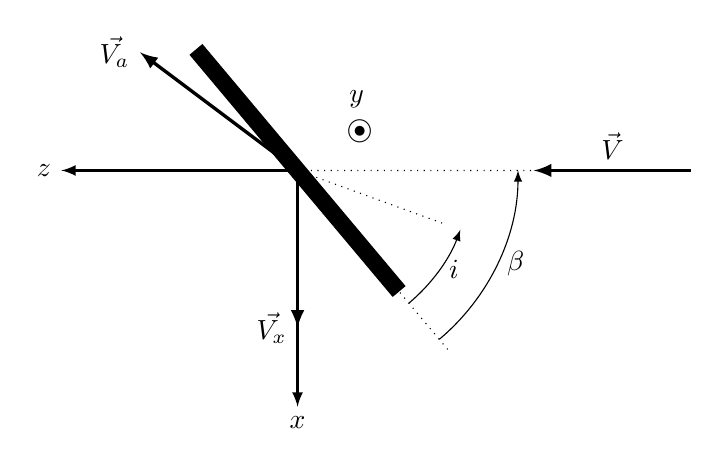
\begin{tikzpicture}
    \draw[-latex,thick] (0,0) -- ++(-3,0)node[left]{$z$};
    \draw[-latex,thick] (0,0) -- ++(0,-3)node[below]{$x$};
    \draw[-latex,very thick] (0,0) -- ++(0,-2) node[left]{$\vec{V_x}$};
    \draw[-latex,very thick] (5,0) -- ++(-2,0) node[midway,above]{$\vec{V}$};

    \draw[-latex,very thick] (0,0) -- ++(-2,1.5) node[left]{$\vec{V_a}$};
    \draw[dotted] (0,0) -- (3,0) (0,0) -- ++(-20:2) (0,0) -- ++(-50:3)
    ;
    \draw[-latex] (-50:2.2) arc(-50:-20:2.2)node[midway, right]{$i$};
    \draw[-latex] (-50:2.8) arc(-50:0:2.8)node[midway, right]{$\beta$};
    \draw[fill=black,rotate around={-50:(0,0)}] (-2,-0.1) rectangle (2,0.1);
    \draw (0.75,0.5) node{{\small$\bigcirc\hspace{-0,75em}\bullet$}} node[above=0.5em]{$y$};
  \end{tikzpicture}
  \caption{Vue de l'élement de pale dans le plan xOz}
\end{figure}
On définit l'angle d'incidence $i$ comme l'ange entre le vent vu par l'élement de pâle ($\vec{V_a}$) et la pale. Pour un angle de calage $\beta$ donné, cet angle est fonction de la vitesse du vent et de la vitesse due à la rotation$V_x$.
On a  donc $\vec{V_a} = \vec{V}-\vec{V_x} $ soit:
\[
  \begin{cases}
    V_a = \sqrt{V^2+(r\Omega)^2}\\
    i = \beta - \arctan\left(\frac{r\Omega}{V}\right)
  \end{cases}
\]
On pose $\lambda = \frac{r\Omega}{V}$ vitesse spécifique du tronçon et on a par exemple l'allure suivante:
\begin{figure}[H]
  \centering
  \begin{tikzpicture}
    \begin{axis}
      [xmin=0,xmax=1,
      ymin=-30,ymax=30,
      samples=51,
      xlabel={$\lambda$},
      ylabel={$i(\frac{\pi}{8},\lambda)$}]
      \addplot[black]{22.5-atan(x)};
    \end{axis}
  \end{tikzpicture}
  \caption{Variation de l'angle d'incidence en degré en fonction de la vitesse spécifique $\lambda$ pour un angle de calage $\beta =\frac{\pi}{8}$.}
  \label{fig:ploti}
\end{figure}


La figure \ref{fig:ploti} représente l'évolution de l'angle d'incidence en fonction de la vitesse spécifique pour un angle de calage donnée. Pour un angle de calage donné et à vitesse de vent donnée, l’angle d’incidence diminue lorsque la vitesse de rotation ou le rayon augmente. Pour un angle de calage et une vitesse de rotation donnés, l’angle d’incidence augmente lorsque la vitesse du vent augmente.
\begin{prop}
En négligeant les effets des frottements, il s’exerce sur cet élément une force de pression $(\d R)$ perpendiculaire à la surface (analogue à la force de pénétration d’un véhicule dans l'air) dont le module s’écrit :
\[
  \d R = kV_a^2.\d S'
\]
où $dS'$ représente la surface de la pale offerte au vent:
\[
  \d S' = l.\sin(i).\d r
\]
d'où:
\[
  \d R = kV_a^2.l\sin(i)\d r
\]
\end{prop}
Il est d’usage de décomposer cette force $(\d R)$ en :

\begin{itemize}
\item  une force dans la direction du vent apparent $(\d T)$ appelée traînée,
\item  une force perpendiculaire à la direction du vent apparent $(\d P)$ appelée portance.
\end{itemize}

\begin{figure}[H]
  \centering
  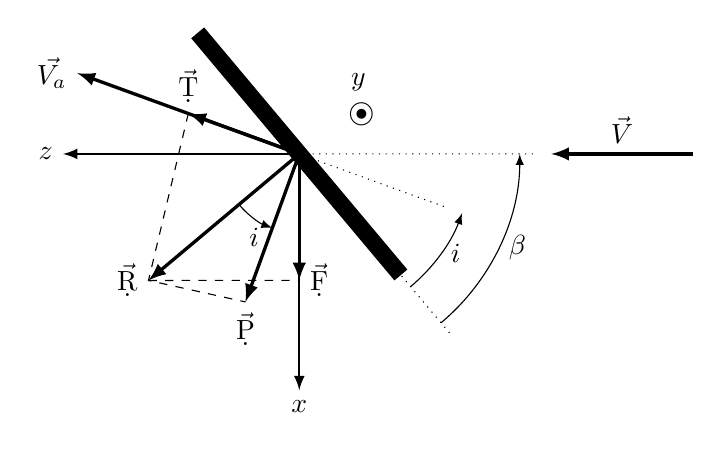
\begin{tikzpicture}
    \draw[-latex,thick] (0,0) -- ++(-3,0)node[left]{$z$};
    \draw[-latex,thick] (0,0) -- ++(0,-3)node[below]{$x$};
    \draw[-latex,very thick] (5,0) -- ++(-1.8,0) node[midway,above]{$\vec{V}$};
    \draw[-latex,very thick] (0,0) -- (220:2.5) node[left]{$\vec{\d R}$};
    \draw[-latex,very thick] (0,0) -- (250:2) node[below]{$\vec{\d P}$};
    \draw[-latex,very thick] (0,0) -- (160:1.5) node[above]{$\vec{\d T}$} ;
    \draw[-latex,very thick] (0,0) -- (0,-1.606) node[right]{$\vec{\d F}$};
    \draw[dashed] (160:1.5) -- (220:2.5) -- (250:2) (220:2.5)-- (0,-1.606);
    \draw[-latex,very thick] (0,0) -- (160:3) node[left]{$\vec{V_a}$};
    \draw[dotted] (0,0) -- (3,0) (0,0) -- (-20:2) (0,0) -- (-50:3)
    ;
    \draw[-latex] (-50:2.2) arc(-50:-20:2.2)node[midway, right]{$i$};
    \draw[-latex] (220:1) arc(220:250:1)node[midway,below]{$i$};
    \draw[-latex] (-50:2.8) arc(-50:0:2.8)node[midway, right]{$\beta$};
    \draw[fill=black,rotate around={-50:(0,0)}] (-2,-0.1) rectangle (2,0.1);
    \draw (0.75,0.5) node{{\small$\bigcirc\hspace{-0,75em}\bullet$}} node[above=0.5em]{$y$};
  \end{tikzpicture}
  \caption{Force motrice $\d F$}
\end{figure}

On en déduit:
\[
  \begin{cases}
    \d T = \d R \sin(i) = kV_a^2.l\sin(i)^2\d r\\
    \d P = \d T = \d R \sin(i) = kV_a^2.l\sin(i)\cos(i)\d r
  \end{cases}
\]
On définit les coefficient de portance $C_L$\footnote{L comme lift} et de trainée $C_D$ \footnote{D comme drag}
\[
  \begin{cases}
    \d T = \frac{1}{2}\rho C_D V_a^2l.\d r \\
    \d P = \frac{1}{2}\rho C_L V_a^2l.\d r
  \end{cases}
\]
\begin{prop}
Dans notre cas les coefficients de trainée et portance sont donc:
\[
  C_D = \frac{2k}{\rho}\sin(i)^2 \text{ et } C_L = \frac{2k}{\rho}\sin(i)\cos(i)
\]
\end{prop}
\begin{figure}[H]
  \centering
  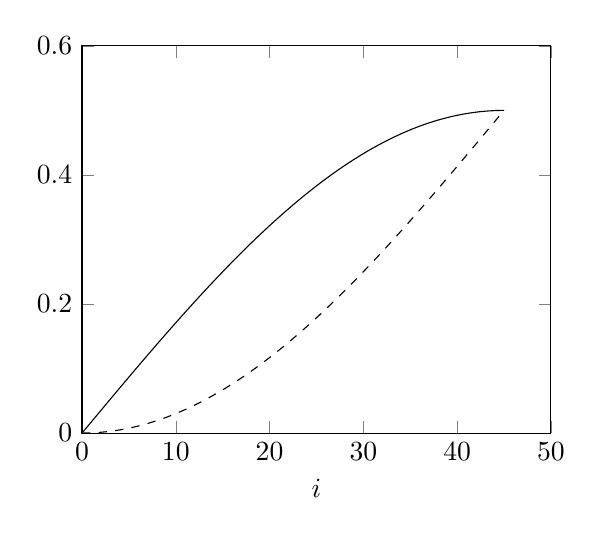
\begin{tikzpicture}
    \def\c{1}
    \begin{axis}
      [height=6.5cm,
      xmin=0,xmax=50,
      ymin=0,ymax=0.6,
      domain=0:45,
      samples=51,
      xlabel={$i$},
      ylabel={}]
      \addplot[black,dashed]{\c*sin(x)^2};
      \addplot[black]{\c*sin(x))*cos(x)};
    \end{axis}
  \end{tikzpicture}
  \caption{Variation des coefficient de portance et de trainée en fonction de l'angle d'incidence}
  \label{fig:plotcoef}
\end{figure}
Les deux forces élémentaires dT et dP vont engendrer une force motrice dF et un couple élémentaire :

\[
 \d C= r.\d F = r\left(\d P.\cos(\beta-i)-\d T.\sin(\beta-i)\right)
\]

On en déduit que la contribution de cet élément à la puissance mécanique est donnée par la relation :
\[
 \d P_m = \d C \Omega =\frac{1}{2}\rho r V_a^2\Omega.l\left(C_L(i).cos(\beta-i)-C_D(i).\sin(\beta-i)\right)dr
\]

où \[V_a^2 = V^2+(\Omega r)^2 \]
et \[i= \beta-\arctan\left(\frac{r\Omega}{V}\right)\]
La figure suivante représente l’allure de la contribution à la puissance mécanique de ce tronçon pour un angle $y$ de calage et une vitesse de vent donnés.

\begin{figure}[H]
  \centering
  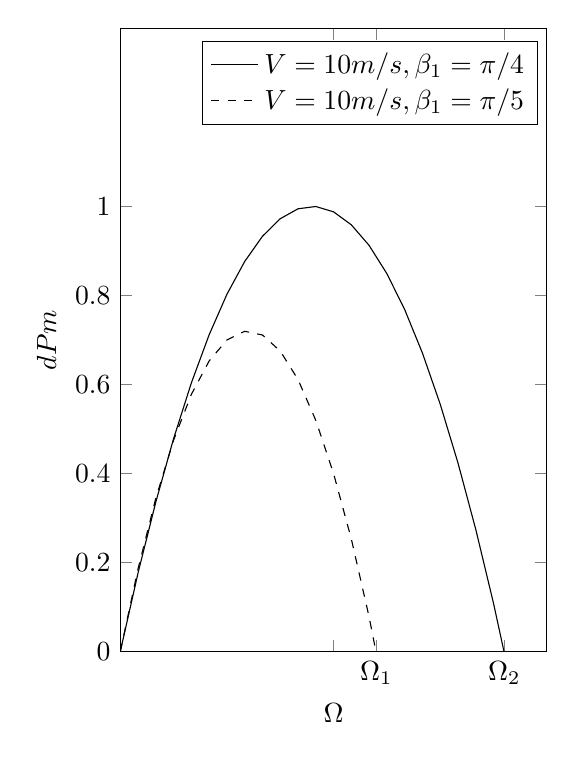
\begin{tikzpicture}
    \begin{axis}
      [xmin=0,xmax=2,ymin=0,ymax=1.4,
      ytick={0,0.2,0.4,0.6,0.8,1},
      height=9.5cm,width=7cm,
      ylabel=$dPm$,xlabel=$\Omega$,
      xtick={1,1.2,1.8},
      xticklabels={,$\Omega_1$,$\Omega_2$},
      domain=0:2]
      \addplot[black] {-x*(x-1.8)/0.81};
      \addlegendentry{$V=10m/s,\beta_1=\pi/4$};
      \addplot[black,dashed] {-x*(x-1.2)*2};
      \addlegendentry{$V=10m/s,\beta_1=\pi/5$};
    \end{axis}
  \end{tikzpicture}
  \caption{Évolution de la puissance en fonction de la vitesse angulaire de rotation pour un angle de calage donné et deux vitesses de vent}
\end{figure}

À vitesse de vent donnée, la puissance passe par un maximum qui dépend de la vitesse du vent. Cette puissance s’annule pour un angle $(i)$ d’incidence nul, soit encore pour :  $\Omega=\frac{V}{r}\tan(\beta)$
\begin{rem}
\begin{itemize}
\item Il faudrait pouvoir adapter la vitesse de rotation de l’hélice à la vitesse du vent pour optimiser la conversion d’énergie cinétique en énergie mécanique.
\item La vitesse angulaire correspondant au maximum de
puissance dépend de la vitesse du vent mais aussi
de r (position du tronçon de pale par rapport à l’axe
de rotation). Il est donc nécessaire de vriller le pro-
fil de la pale($\beta$ est fonction de $r$) pour optimiser la
conversion.
\item Le calcul de la puissance totale se fait en
intégrant la puissance élémentaire de 0 à R, rayon
de l’hélice :
\[
P_m = \int_{0}^{R}\d P_m
\]
\end{itemize}
\end{rem}
\subsection{Pale réelle}
\subsection{Comparaison des différents types de turbines}
\subsection{Réglage de la conversion}
\subsection{Exemple de caractéristiques}








\end{document}

%%% Local Variables:
%%% mode: latex
%%% TeX-master: "main"
%%% End:
